\chapter{Linear Models for Classification}
\label{ch:classification}

\chapterguide%
  {\chapref{ch:regression}, \chapref{ch:training}, the gradient-descent walk of \secref{sec:gradient-descent}, and probability from \chapref{ch:statistics}.}
  {explain why a line cannot output a probability; turn a score into a probability with the sigmoid; compute log loss by hand and say why it beats squared error; fit a logistic model by gradient descent; move a threshold on purpose; and compare softmax, LDA, QDA and the perceptron.}

The tutor's next question has a different kind of answer: will this student pass? A mark can be any number, but a pass is yes or no. And because a wrong answer costs something (a student who needed help gets none, or tutoring hours go to a student who was fine), the tutor wants more than a verdict. The tutor wants to know how sure the model is.

\section{Why not just use linear regression?}

Look at the lectures column against who passed. Students who attended 3 and 5 lectures failed, and those who attended 9 or more passed. In between it is mixed: B passed with 6, and A failed with 8. Write fail as 0 and pass as 1, and fit the same straight line as before:
\[
  \hat{y}=0.100\times\text{lectures}-0.136.
\]
The fit runs without complaint until you read what it says. At 13 lectures the answer is 1.158, a 116\% chance. At 0 lectures it is $-0.136$, a chance of minus 14\%. A straight line has no idea that a probability must stop at 0 and at 1 (\figref{fig:s-curve}).

\section{The dimmer switch}

\begin{analogy}
A light switch is off or on, like our labels. A dimmer sweeps smoothly from dark to full brightness, and however far you turn the dial, the light cannot go below off or above fully on. Keep the straight line as the dial, and pass its output through a dimmer. The dial position is the \term{score}, and the brightness is the probability.
\end{analogy}

That dimmer is the \term{sigmoid}, a name that just means S-shaped:
\[
  \sigma(z)=\frac{1}{1+e^{-z}},
  \qquad
  z=w\,x+b.
\]
Here $e\approx2.72$ is a fixed number. A score of 0 gives exactly 0.5, because $e^0=1$. A score of 2 gives 0.881 and a score of $-2$ gives 0.119. The sign of the score picks the side, and its size sets the confidence. The combined model is called \term{logistic regression}. The name is confusing, since it does classification, but it is the old name and everyone uses it.

\begin{utpfig}[Squashing the line]{Pass or fail against lectures attended. The straight line leaves the possible range at both ends, shown in red. The fitted S-curve stays between 0 and 1 and crosses 0.5 at 6.30 lectures. Student A failed with 8 lectures, and student B passed with 6.}{fig:s-curve}
\begin{tikzpicture}
\begin{axis}[logaxis, width=0.80\linewidth, height=6.2cm, xlabel={lectures attended}, ylabel={model's answer}, xmin=0, xmax=14.5, ymin=-0.25, ymax=1.35,
  ytick={0,0.5,1}, legend style={at={(0.03,0.95)},anchor=north west}, clip=true]
\fill[UTPPaleRed] (axis cs:0,1) rectangle (axis cs:14.5,1.35);
\fill[UTPPaleRed] (axis cs:0,-0.25) rectangle (axis cs:14.5,0);
\addplot[draw=UTPOrange,thick,domain=0:14.5] {0.1*x-0.136}; \addlegendentry{straight line}
\addplot[draw=UTPBlue,very thick,domain=0:14.5,samples=80] {1/(1+exp(-(0.7885*(x-8)+1.3371)))}; \addlegendentry{S-curve}
\addplot[draw=UTPMuted,dashed,domain=0:14.5,forget plot] {0.5};
\addplot[logdots,forget plot] table[x=lectures,y=passed,meta=name] {\studylog};
\end{axis}
\end{tikzpicture}
\end{utpfig}

\section{From probabilities to odds to a linear model}

The sigmoid has a neat reverse reading, which explains what the slope means. \term{Odds} are $p/(1-p)$: $p=0.75$ gives odds of 3. Their logarithm, the \term{logit}, spans the whole number line, and logistic regression assumes it is linear in the features:

\begin{utptable}
\begin{tabularx}{0.78\linewidth}{@{}>{\bfseries\leavevmode\color{UTPNavy}}X X X@{}}
\toprule
\rowcolor{UTPPaleBlue!92}
\utpth{Probability} & \utpth{Odds} & \utpth{Read aloud} \\
\midrule
$50\%$ & $1:1$ & equally likely either way \\
$75\%$ & $3:1$ & three chances for, one against \\
$90\%$ & $9:1$ & nine chances for, one against \\
\bottomrule
\end{tabularx}
\end{utptable}

\[
  \log\frac{p}{1-p}
  =\beta_0+\bm{\beta}^{\mathsf T}\bm{x},
  \qquad\text{equivalently}\qquad
  P(Y=1\given\bm{x})=\sigma(\beta_0+\bm{\beta}^{\mathsf T}\bm{x}).
\]

\begin{utpfig}[The sigmoid]{The sigmoid maps an unrestricted score to a probability. Scores near zero give probabilities near $0.5$; large positive or negative scores give confident answers.}{fig:sigmoid}
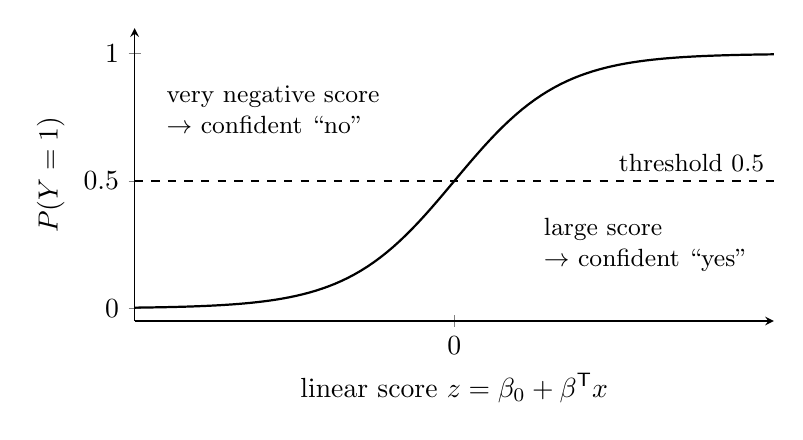
\begin{tikzpicture}
\begin{axis}[
  width=0.80\linewidth, height=5.3cm,
  axis lines=left,
  xlabel={linear score $z=\beta_0+\bm{\beta}^{\mathsf T}\bm{x}$},
  ylabel={$P(Y=1)$},
  ytick={0,0.5,1}, xtick={0},
  domain=-6:6, samples=100, ymin=-0.05, ymax=1.1, clip=false
]
\addplot[thick] {1/(1+exp(-x))};
\draw[dashed] (axis cs:-6,0.5) -- (axis cs:6,0.5)
  node[above left, font=\small] {threshold $0.5$};
\node[font=\small, align=left] at (axis cs:3.6,0.25) {large score\\$\rightarrow$ confident ``yes''};
\node[font=\small, align=left] at (axis cs:-3.4,0.78) {very negative score\\$\rightarrow$ confident ``no''};
\end{axis}
\end{tikzpicture}
\end{utpfig}

A unit increase in $x_j$ multiplies the odds by $e^{\beta_j}$, holding other features fixed. So $\beta_j=0.7$ roughly doubles the odds and $-0.7$ roughly halves them. The effect on the probability depends on where you start, because the curve is steep in the middle and flat at the ends.

\begin{workedexample}
Suppose a pass/fail model based on hours studied has $\beta_0=-4$ and $\beta_1=0.08$.
A student with $x=60$ hours has score $z=-4+0.08\times 60=0.8$ and pass probability $\sigma(0.8)\approx 0.69$.
A student with $x=30$ hours has $z=-1.6$ and $\sigma(-1.6)\approx 0.17$.
Each additional hour multiplies the odds of passing by $e^{0.08}\approx 1.083$ --- about an $8\%$ increase in the odds, regardless of the starting point.
\end{workedexample}

\section{The loss: confident and wrong}

We need to score a probability. Reaching for squared error again seems natural, so try it on a student who failed, with the model giving three different chances of passing.

\begin{workedexample}
\centering\small
\begin{tabular}{@{}lccc@{}}
\toprule
\rowcolor{UTPPaleBlue!92}
\utpth{Chance given to ``pass''} & \utpth{The lean} & \utpth{Squared error} & \utpth{Log-loss fee} \\
\midrule
0.60 & mild & $0.60^2=0.360$ & $-\ln(0.40)=0.916$ \\
0.90 & strong & $0.90^2=0.810$ & $-\ln(0.10)=2.303$ \\
0.99 & certain & $0.99^2=0.980$ & $-\ln(0.01)=4.605$ \\
\bottomrule
\end{tabular}
\par\raggedright
\medskip
Squared error cannot pass 1, so being certain and wrong costs 0.98, barely more than the 0.81 for merely leaning that way. It has run out of room exactly where the mistake is worst. The fee on the right has no ceiling.
\end{workedexample}

The better score is \term{log loss}, also called \term{cross-entropy}: the fee is minus the logarithm of the probability the model gave to what actually happened.
\[
  \mathcal{L}(y,p)
  =-[y\log p+(1-y)\log(1-p)].
\]
A probability is below 1, so its logarithm is negative, and the minus sign turns that into a positive fee. A sure right answer is almost free. A sure wrong answer is ruinous. A model that says 50\% pays 0.693 whichever way the case goes (\figref{fig:fees}).

\begin{utpfig}[The fee for each probability]{The log-loss fee against the chance given to ``pass'', for a student who passed and a student who failed. The two curves cross at 0.5, where the fee is 0.693, and each climbs without limit as the model grows confident and wrong. Squared error for a failing student is shown for comparison.}{fig:fees}
\begin{tikzpicture}
\begin{axis}[logaxis, width=0.70\linewidth, height=5.4cm, xlabel={chance given to ``pass''}, ylabel={fee}, xmin=0, xmax=1, ymin=0, ymax=5,
  legend style={at={(0.5,0.97)},anchor=north}]
\addplot[draw=UTPBlue,thick,domain=0.007:1,samples=80] {-ln(x)}; \addlegendentry{student passed: $-\ln p$}
\addplot[draw=UTPOrange,thick,domain=0:0.993,samples=80] {-ln(1-x)}; \addlegendentry{student failed: $-\ln(1-p)$}
\addplot[draw=UTPMuted,dashed,domain=0:1] {x^2}; \addlegendentry{squared error, student failed}
\end{axis}
\end{tikzpicture}
\end{utpfig}

\section{The optimizer: walking down}

Unlike squared error on a line, log loss has no exact formula for its best $w$ and $b$, so the model has to walk. Everything you need is already here: the model, the loss, and the gradient-descent rule from \secref{sec:gradient-descent}. The two slopes work out neatly: for each row, the slope is simply the prediction minus the truth, $(p_i-y_i)$, weighted by the feature.
\[
  \frac{\partial J}{\partial w}=\frac{1}{n}\sum_i(p_i-y_i)\,x_i,
  \qquad
  \frac{\partial J}{\partial b}=\frac{1}{n}\sum_i(p_i-y_i).
\]
We center the lectures on 8, because that keeps the numbers small. Nothing else changes. The whole fit, in code:

\lstinputlisting[style=utppython,firstline=61,lastline=80]{all_experiments/book_checks/demo_study_log.py}

\begin{workedexample}
At the start, $w=b=0$, so every $p$ is 0.5. The formula gives a slope of $-1.0000$ for $w$. Nudging $w$ by 0.001 and remeasuring the loss gives $-0.9988$, so the formula checks out. With a learning rate of 0.1:

\medskip
\centering\small
\begin{tabular}{@{}cccc@{}}
\toprule
\rowcolor{UTPPaleBlue!92}
\utpth{Step} & \utpth{$w$} & \utpth{$b$} & \utpth{Log loss} \\
\midrule
1 & 0.1000 & 0.0200 & 0.6011 \\
10 & 0.4497 & 0.1612 & 0.4285 \\
100 & 0.6819 & 0.8664 & 0.3528 \\
500 & 0.7827 & 1.3163 & 0.3430 \\
2000 & 0.7885 & 1.3371 & 0.3430 \\
\bottomrule
\end{tabular}
\par\raggedright
\medskip
The loss falls fast and then barely moves, because the walk has reached the flat bottom.
\end{workedexample}

\section{What the fitted model says}

Follow one student all the way through. Student A attended 8 lectures, so the centered value is 0. The score is $0.7885\times0+1.3371=1.337$, and the chance of passing is $\sigma(1.337)=0.792$. The score can be any number at all; the probability can never leave 0 to 1.

\begin{utptable}
\centering
\begin{tabular}{@{}>{\bfseries\color{UTPNavy}}ccccccc@{}}
\toprule
\rowcolor{UTPPaleBlue!92}
\utpth{Student} & \utpth{Lectures} & \utpth{Passed?} & \utpth{Score} & \utpth{Chance} & \utpth{Verdict} & \utpth{Right?} \\
\midrule
J & 3 & no & $-2.605$ & 0.069 & fail & yes \\
I & 5 & no & $-1.028$ & 0.263 & fail & yes \\
B & 6 & yes & $-0.240$ & 0.440 & fail & \textbf{no} \\
C & 7 & yes & 0.549 & 0.634 & pass & yes \\
A & 8 & no & 1.337 & 0.792 & pass & \textbf{no} \\
D & 9 & yes & 2.126 & 0.893 & pass & yes \\
H & 10 & yes & 2.914 & 0.949 & pass & yes \\
E & 11 & yes & 3.703 & 0.976 & pass & yes \\
G & 12 & yes & 4.491 & 0.989 & pass & yes \\
F & 13 & yes & 5.280 & 0.995 & pass & yes \\
\bottomrule
\end{tabular}
\end{utptable}

The model is right on 8 of 10. Its two mistakes differ in kind. Student B was a near thing at 0.44, and pays a fee of 0.820. Student A is the expensive one: the model was 79\% sure, and A failed, for a fee of 1.570. A's two hours of study are not visible to a model that sees only lectures, which is a reminder that a model can be only as good as its columns.

Each extra lecture multiplies the odds of passing by $e^{0.7885}=2.20$. The score is zero, and the chance exactly 0.5, at $8-1.3371/0.7885=6.30$ lectures. That point is the \term{decision boundary}.

\subsection{The decision boundary and the threshold}

At threshold $0.5$, class~1 means $z\ge0$, giving the boundary $\beta_0+\bm{\beta}^{\mathsf T}\bm{x}=0$. With two features that boundary is a straight line, and with more it is a flat plane, which is why logistic regression is called a linear classifier even though its output curve is not straight.

The probability and the decision are separate objects. The model supplies the first. The threshold is a policy, chosen to reflect error costs on validation or out-of-fold predictions (\chapref{ch:evaluation}). These are Lab~2's results for one fitted model on the 40,687 hotel bookings of 2017, Part~C, where a flagged booking is treated as a likely cancellation:

\begin{utptable}
\begin{tabularx}{\linewidth}{@{}>{\bfseries\leavevmode\color{UTPNavy}}m{0.14\linewidth}ccccX@{}}
\toprule
\rowcolor{UTPPaleBlue!92}
\utpth{Threshold} & \utpth{Flagged} & \utpth{Precision} & \utpth{Recall} & \utpth{Cancellations missed} & \utpth{What changed} \\
\midrule
0.30 & 20,052 & 0.61 & 0.77 & 3,558 & many bookings flagged; most cancellations caught \\
0.50 & 11,095 & 0.78 & 0.55 & 7,129 & the default \\
0.70 & 4,822 & 0.96 & 0.29 & 11,117 & few flagged, almost all right; most cancellations missed \\
\bottomrule
\end{tabularx}
\end{utptable}

Choose the operating point from a stated cost or capacity. Then refit on all training data and assess the locked rule on the test set once.

\subsection{Regularization}

Use $L_1$ or $L_2$ penalties with appropriately scaled features and validation-selected strength (\chapref{ch:regression}). Regularization also stops coefficients diverging on perfectly separable data, where a steeper S always scores better and the walk would never end. Lab~2's grid search tunes this strength as $C$, and in scikit-learn a larger $C$ means a weaker penalty.

\recipecard{Logistic regression}{The straight line's score, squashed by the sigmoid into a probability.}{Log loss, which is very large when the model is confident and wrong.}{Gradient descent or a Newton-type method. No exact formula exists.}

\section{Softmax regression for multiple classes}

For $K$ classes, each class $k$ receives its own weight vector, and the \term{softmax} function converts the $K$ linear scores into probabilities:
\[
  P(Y=k\given\bm{x})
  =\frac{\exp(\bm{\beta}_k^{\mathsf T}\bm{x})}
        {\sum_{j=1}^{K}\exp(\bm{\beta}_j^{\mathsf T}\bm{x})}.
\]
Exponentiating and normalizing preserves score order and makes probabilities sum to one. Training minimizes $\mathcal{L}=-\log P(Y=y\given\bm{x})$.

\term{One-vs-rest} trains $K$ binary classifiers, one class against all others, and predicts the highest-scoring class.

\begin{utpfig}[Softmax]{Softmax turns class scores into probabilities. Scores 1.2, 3.4 and 2.0 become 0.08, 0.74 and 0.18: the order is preserved and the probabilities add to one.}{fig:softmax}
\begin{tikzpicture}[
  node distance=0.36cm and 0.62cm,
  sc/.style={draw=UTPBlue,fill=UTPPaleBlue,rounded corners=1.2mm,minimum width=1.55cm,minimum height=0.6cm,align=center,font=\scriptsize\color{UTPNavy}},
  pr/.style={draw=UTPGreen,fill=UTPPaleTeal,rounded corners=1.2mm,minimum width=1.55cm,minimum height=0.6cm,align=center,font=\scriptsize\color{UTPNavy}},
  arr/.style={-{Stealth[length=2mm]},thick,draw=UTPTeal}
]
\node[sc] (s1) {cat: $1.2$};
\node[sc,below=of s1] (s2) {dog: $3.4$};
\node[sc,below=of s2] (s3) {fox: $2.0$};
\node[draw=UTPOrange,fill=UTPPaleOrange,rounded corners=2mm,minimum height=2.5cm,minimum width=1.9cm,align=center,font=\scriptsize\bfseries\color{UTPNavy},right=1.0cm of s2] (sm) {softmax\\[0.15em]\scriptsize\mdseries exponentiate,\\then divide by\\the total};
\node[pr,right=1.0cm of sm] (p2) {dog: $0.74$};
\node[pr,above=of p2] (p1) {cat: $0.08$};
\node[pr,below=of p2] (p3) {fox: $0.18$};
\draw[arr] (s1.east) -- (sm.west); \draw[arr] (s2.east) -- (sm.west); \draw[arr] (s3.east) -- (sm.west);
\draw[arr] (sm.east) -- (p1.west); \draw[arr] (sm.east) -- (p2.west); \draw[arr] (sm.east) -- (p3.west);
\node[font=\scriptsize\itshape\color{UTPMuted},below=0.3cm of p3] {always adds to 1.00};
\end{tikzpicture}
\end{utpfig}

\begin{workedexample}
For scores $1.2,\ 3.4,\ 2.0$, the exponentials are $3.32,\ 29.96,\ 7.39$, which add to $40.67$. Dividing gives $0.082,\ 0.737,\ 0.182$.
\end{workedexample}

\begin{keyidea}
Softmax preserves score order while normalizing exponentials to a probability distribution.
\end{keyidea}

\section{Ordered categories are not ordinary multiclass labels}
\label{sec:ordinal-labels}

\term{Ordinal labels} have order, such as low $<$ medium $<$ high. Softmax ignores order; numerical coding for regression assumes meaningful gaps.

\begin{utptable}
\begin{tabularx}{\linewidth}{@{}m{0.25\linewidth}X@{}}
\toprule
\rowcolor{UTPPaleBlue!92}
\utpth{Approach} & \utpth{When it makes sense} \\
\midrule
Ordinary multiclass classifier & Use when categories are genuinely unordered or when order is irrelevant to the decision. \\
Ordinal model / order-aware loss & Prefer when confusing adjacent levels is meaningfully less serious than confusing the two extremes. \\
Regression on integer codes & Use only when the numerical spacing itself is defensible; do not use it merely because the labels can be numbered. \\
\bottomrule
\end{tabularx}
\end{utptable}

Choose order-aware methods or metrics when warranted, and validate whether they help.

\section{Linear discriminant analysis}

Logistic regression learns the boundary directly. Another way to classify is to describe each class by itself, and then ask which description fits a new row better.

Logistic regression is \term{discriminative}: it models $P(y\given\bm{x})$. \term{Linear discriminant analysis (LDA)} is \term{generative}: it models each class's feature distribution and applies Bayes' theorem.

LDA assumes Gaussian classes with means $\bm\mu_k$, shared covariance $\Sigma$, and priors $\pi_k$. Choose the largest discriminant score:
\[
  \delta_k(\bm{x})
  =\bm{x}^{\mathsf T}\Sigma^{-1}\bm{\mu}_k
  -\tfrac{1}{2}\bm{\mu}_k^{\mathsf T}\Sigma^{-1}\bm{\mu}_k
  +\log\pi_k.
\]
Estimate priors from frequencies, means within classes, and covariance from pooled within-class variation. Linear dependence on $\bm x$ gives flat boundaries.

\begin{workedexample}
On the lectures column of the log, passing students average 9.71 lectures and failing students 5.33, with a pooled variance of 6.51. With equal class sizes the boundary would be the midpoint, 7.52. Passing is more common here (7 of 10), and the prior moves the boundary down to 6.26, close to logistic regression's 6.30.
\end{workedexample}

\begin{intuition}
With equal-shaped Gaussian class densities, the tie boundary is linear; class priors shift its position.
\end{intuition}

When to prefer which:

\begin{itemize}
  \item LDA can be stable on small datasets when Gaussian assumptions are reasonable.
  \item Logistic regression assumes less about the features and is more robust when classes are far from Gaussian (heavy tails, strong outliers, many binary features).
  \item LDA also finds up to $K-1$ supervised projection directions for $K$ classes (\chapref{ch:dimred}).
\end{itemize}

\term{Quadratic discriminant analysis (QDA)} drops the shared-covariance assumption and gives each class its own $\Sigma_k$. The boundaries become curved (quadratic), which is more flexible but requires estimating many more parameters --- QDA needs considerably more data per class to stay reliable.

\section{The perceptron}

The perceptron is the simplest trainer there is, and the ancestor of the neural networks in \chapref{ch:deep}. It has no probabilities and no loss curve: when it makes a mistake it moves the line, and when it does not, it does nothing.

The \term{perceptron} predicts $\hat y=\operatorname{sign}(\bm w^{\mathsf T}\bm x+b)$ for $y\in\{-1,+1\}$. For each misclassified example, update
\[
  \bm{w}\leftarrow\bm{w}+\eta\,y_i\,\bm{x}_i,
  \qquad
  b\leftarrow b+\eta\,y_i.
\]
Correct predictions cause no update. Separable data yields convergence; otherwise convergence is not guaranteed. The boundary depends on the training path and supplies no probabilities.

\begin{workedexample}
Four points: $(2,2)$ and $(0,2)$ are $+1$; $(-1,-1)$ and $(1,-1)$ are $-1$. Start with $\bm{w}=(0,0)$, $b=0$ and $\eta=1$.
\begin{description}
  \item[$(2,2)$] The score is 0, which counts as a mistake, so $\bm{w}=(2,2)$ and $b=1$.
  \item[$(-1,-1)$] The score is $-3$, which is correct, so nothing changes.
  \item[$(1,-1)$] The score is $+1$, a mistake, so $\bm{w}=(1,3)$ and $b=0$.
  \item[$(0,2)$] The score is $+6$, which is correct.
\end{description}
A second pass makes no mistakes, so training stops with $\bm{w}=(1,3)$ and $b=0$.
\end{workedexample}

\section{Choosing among linear classifiers}

\begin{utptable}
\begin{tabular}{@{}p{0.22\linewidth}p{0.34\linewidth}p{0.34\linewidth}@{}}
\toprule
\rowcolor{UTPPaleBlue!92}
\utpth{Model} & \utpth{Useful strengths} & \utpth{Important limitations} \\
\midrule
Logistic regression & Strong probability baseline, convex training, interpretable odds ratios & Linear boundary; probabilities can still be miscalibrated under misspecification or shift \\
LDA & Very fast, stable on small data, gives class-separating directions & Assumes Gaussian classes with shared covariance \\
QDA & Curved boundaries, per-class covariance & Many parameters; needs much more data \\
Perceptron & Simplest possible trainer; historically important & No probabilities; unreliable when classes overlap \\
\bottomrule
\end{tabular}
\end{utptable}

\begin{keyidea}
Logistic regression fits conditional probabilities; LDA models class distributions; the perceptron updates after mistakes. All use flat boundaries, while QDA's separate covariance matrices allow curves.
\end{keyidea}

\begin{modelcard}{Linear Classifiers - Quick Guide}
\begin{tabularx}{\linewidth}{@{}>{\bfseries\leavevmode\color{UTPNavy}}p{0.24\linewidth}X@{}}
Best when & A linear boundary is reasonable, fast prediction matters, or coefficients need to be interpreted. \cr
Start with & Logistic regression for probabilities; softmax regression for several classes. \cr
Preprocessing & Encode categories, standardize numerical features for regularization, and handle imbalance with suitable metrics or weights. \cr
Main controls & Regularization strength, penalty type, and the probability threshold used for decisions. \cr
Watch for & Nonlinear class structure, poorly calibrated probabilities, rare classes, and causal over-interpretation (\secref{sec:correlation}). \cr
\end{tabularx}
\end{modelcard}

\begin{workedexample}
For an ``hours studied'' coefficient of $0.62$, each extra hour multiplies passing odds by $e^{0.62}\approx1.86$, holding other features fixed. The probability increase depends on the starting probability.
\end{workedexample}

\begin{tryit}
Fit logistic regression and obtain out-of-fold training probabilities. Sweep thresholds from 0.05 to 0.95 in steps of 0.05; plot precision against recall without using test data.
\end{tryit}

\begin{debugtask}
A teammate lowers the probability threshold until test-set recall reaches the desired value, then reports that same test recall as final performance. Explain the leakage in model selection and show where threshold tuning belongs instead.
\end{debugtask}

\begin{decisionmemo}
For a rare positive class, choose between an unweighted logistic model, class weighting, and a lower decision threshold. State which quantity each intervention changes, which validation metric you would inspect, and why the three options are not interchangeable.
\end{decisionmemo}

\begin{chapterrecap}
\begin{itemize}
  \item A straight line on 0/1 labels leaves the range of a probability, so logistic regression passes its score through the sigmoid, a dimmer that stops at 0 and 1.
  \item The score's sign picks the side and its size sets the confidence. A unit of a feature multiplies the odds by $e^{\beta}$.
  \item Log loss charges minus the log of the probability given to what happened, so confident and wrong is ruinous. Squared error cannot punish it enough.
  \item There is no formula, so the model walks down by gradient descent. Each row's slope is the prediction minus the truth, weighted by the feature.
  \item The probability and the threshold are separate. Softmax extends the model to many classes; LDA models each class; the perceptron just corrects its mistakes.
\end{itemize}
\end{chapterrecap}

\begin{quickcheck}
\begin{enumerate}
  \item A score is exactly 0. What probability does the sigmoid give, and why?
  \item With the fitted model, what chance of passing does a student with 7 lectures get, and which side of a 0.5 threshold is that?
  \item A model gives 0.95 to a case that turns out negative. What does it pay in log loss? And for a case that turns out positive?
  \item Why is logistic regression called a linear classifier even though it outputs a nonlinear sigmoid probability?
  \item Why should the probability model and the operational classification threshold be treated as separate objects?
  \item What changes when binary logistic regression is extended to a multiclass softmax model?
\end{enumerate}
\end{quickcheck}

\begin{checkanswers}
\begin{enumerate}
  \item 0.5, because $e^0=1$, so $1/(1+1)=0.5$. The two limits, 0 and 1, are approached but never reached.
  \item 0.634, from a score of 0.549. That is above 0.5, so the verdict is pass, and student C did pass.
  \item Negative case: $-\ln(0.05)=3.00$. Positive case: $-\ln(0.95)=0.05$.
  \item The decision boundary, where the score equals zero, is a flat line or plane in feature space. The sigmoid only maps the score to a probability, and it does not bend the boundary.
  \item The fitted model describes how likely each outcome is, which stays the same however it is used. The threshold is a choice about costs and capacity, which can change without refitting.
  \item Each class gets its own weight vector and score, and softmax turns the scores into probabilities that add to one. Binary logistic regression is the two-class special case.
\end{enumerate}
\end{checkanswers}

\labsection{2}{Supervised learning I: regression, classification, and the workflow}{sec:lab02-supervised-workflow}

\begin{labproject}{A regression problem, two classification problems, and saved models at the end}
\textbf{Read first.} Chapters~\ref{ch:learning}--\ref{ch:classification}.\\
\textbf{Goal.} Fit regression and classification pipelines on messy data, validate in date order where time matters, choose thresholds and hyperparameters on purpose, test once, and save models that can be loaded and used.\\
\textbf{Scenario.} Three commissions: a used-car dealer wants asking prices estimated from a listing, a hotel group wants to know which bookings will be cancelled so it can resell rooms without turning guests away, and a telecom company wants a churn model it can hand to its call centre. Then the models must leave the notebook as files.\\
\textbf{Data.} In \texttt{all\_datasets/\allowbreak supervised/}: \texttt{used\_cars/\allowbreak used\_cars.zip}, 150,000 car listings collected from Cars.com in October 2026; \texttt{hotel\_bookings/\allowbreak hotel\_bookings.zip}, the hotel bookings from Lab~1; and \texttt{telco\_customer\_churn/\allowbreak telco\_customer\_churn.csv}, the telecom customers from Lab~1. Each folder's \texttt{README.md} is its data card.\\
\textbf{Notebook.} \texttt{all\_experiments/\allowbreak lab02\_supervised\_workflow/\allowbreak lab02\_supervised\_workflow\_worked.ipynb}, with \texttt{predict\_churn.py} and a README beside it.\\
\textbf{Hand in.} The executed notebook, \texttt{results/lab02/}, the model files and a decision memo, as listed in the checklist at the end of this sheet.
\end{labproject}

\labroadmap{Your map of this lab}{
      A & Tidy the car listings, predict prices, read the coefficients and the residuals & 2--5 \\
      B & Validate hotel cancellations in date order, and see what a shuffled split hides & 6--8 \\
      C & Beat a baseline, read probabilities, and choose a threshold by cost & 9--12 \\
      D & Tune the churn model with cross-validation, then open the test set once & 13--14 \\
      E & Save the models with a card, reload them and use them & 15--16 \\
      Finish & Save the evidence; then model log prices and write an overbooking memo & 17--19 \\
      After & Your-turn tasks, expected findings, troubleshooting and the two checklists & --- \\
}

\begin{labmode}
\begin{enumerate}
  \item Activate your course environment and confirm the three data files are in \texttt{all\_datasets/\allowbreak supervised/}.
  \item From the course folder, start Jupyter, open the notebook, and choose \textbf{Restart Kernel and Run All Cells}. It takes under a minute.
\end{enumerate}
\begin{lstlisting}[style=utpterminal]
jupyter lab
\end{lstlisting}
Prefer a plain script? From the course folder, \texttt{python all\_experiments/\allowbreak lab02\_supervised\_workflow/\allowbreak lab02\_supervised\_workflow\_worked.py} runs the same code and writes the same evidence.
\end{labmode}

\labroutine

\begin{yourturn}
\textbf{Warm-up on paper.} Do these before opening the notebook; the code will check you.
\begin{enumerate}
  \item True values $10,20,30,40$ and predictions $12,18,30,50$. Compute MAE and RMSE. Why is RMSE larger? (MAE 3.5, RMSE about 5.2.)
  \item Question~9's logistic model at threshold 0.50 flags 2017 bookings as likely cancellations with $TP=8{,}616$, $FP=2{,}479$, $FN=7{,}129$ and $TN=22{,}463$. Compute precision, recall and accuracy. Then predict: if the threshold rises to 0.70, which of these four counts can only grow, and which can only shrink?
\end{enumerate}
\end{yourturn}

\begin{labquestion}{1}{Setup}
Run this first, and keep this kernel for the later questions. Every lab starts the same way. \texttt{start\_lab()}, from \texttt{all\_experiments/\allowbreak course\_setup.py}, finds the course folder and returns the three folders the lab uses: \texttt{DATA} to read from, \texttt{RESULTS} and \texttt{MODELS} to write to. The imports in between are grouped by what they are for. \texttt{make\_preprocess} is the same helper as in Lab~1: median imputation and scaling for numbers, most-frequent imputation and one-hot encoding for categories.
\end{labquestion}
\begin{labanswer}
\lstinputlisting[style=utppython,firstline=11,lastline=51]{all_experiments/lab02_supervised_workflow/lab02_supervised_workflow_worked.py}
\begin{refoutput}
\begin{lstlisting}[style=utpterminal]
course folder: MACHINE LEARNING
reads all_datasets/, writes results/lab02/ and models/
\end{lstlisting}
\end{refoutput}
\end{labanswer}

\labpartopen{Part A}{Regression: ordinary least squares versus ridge}{Questions 2--5 \textbullet\ Data: used-car listings from Cars.com}{Tidy real listings, predict used-car prices with a straight-line model, read its coefficients, and see where it fails.}

\begin{labquestion}{2}{Read the car listings, tidy them, and split}
Each row is one car with a numeric label, \texttt{price\_usd}, so this is regression. Three fixed rules, chosen before any model, keep used cars with a believable price (\$1,000 to \$200,000) and a real odometer reading. Sellers also type the same thing many ways, so \texttt{tidy()} maps the spellings of drivetrain and fuel to a few groups. Two models will share the pipeline and the split; the only difference is ridge's penalty on large coefficients. The car's \texttt{model} (F-150, Camry and over a thousand others) is kept aside for now, and a Your-turn task brings it in.
\end{labquestion}
\begin{labanswer}
\lstinputlisting[style=utppython,firstline=53,lastline=87]{all_experiments/lab02_supervised_workflow/lab02_supervised_workflow_worked.py}
\begin{refoutput}
\begin{lstlisting}[style=utpterminal]
shape: (150000, 19)
stock_type
Used    79262
New     70738
used listings kept: 77,646 of 79,262
spellings before tidying: drivetrain 21  fuel 31
{'AWD': 28787, 'FWD': 18290, '4WD': 17310, 'RWD': 9008, None: 4251}
{'gasoline': 63296, None: 5474, 'electric': 3007, 'hybrid': 2986, 'diesel': 2160,
 'flex fuel': 594, 'plug-in hybrid': 129}
62116 listings to train on and 15530 to validate
\end{lstlisting}
\end{refoutput}

\textbf{What it means.} The rules drop 1,616 used listings, among them 295 with no price shown, 712 priced above \$200,000 (24 of them in the millions) and 659 with 100 miles or fewer on the clock; a few break two rules. Tidying turns 21 spellings of the drivetrain and 31 of the fuel into four and six groups; what matches no group (``2WD'', ``Unknown'', a blank) becomes a gap that the pipeline's imputer fills. Every rule is fixed and reads no label, so it may run before the split. The listings were collected on one day, so a random 80/20 split is honest here.
\end{labanswer}

\begin{labquestion}{3}{Fit OLS and ridge}
Three scores per model. MAE is the typical miss in dollars. RMSE weights big misses more, so when it is much larger than MAE a few predictions are badly wrong. $R^2$ is the share of the price's variation the model explains. Always guessing the training mean is the baseline both must beat.
\end{labquestion}
\begin{labanswer}
\lstinputlisting[style=utppython,firstline=89,lastline=107]{all_experiments/lab02_supervised_workflow/lab02_supervised_workflow_worked.py}
\begin{refoutput}
\begin{lstlisting}[style=utpterminal]
always the training mean: MAE 15408

linear regression          ridge
MAE: 9009                  MAE: 9062
RMSE: 14336                RMSE: 14427
R2: 0.575                  R2: 0.569
\end{lstlisting}
\end{refoutput}

\textbf{What it means.} Both models cut the typical miss from \$15,400 to about \$9,000, and regularization did not help: with 62,116 rows the plain model is already stable. RMSE is about 60\% above MAE, so some cars are missed by far more than the typical amount; Question~5 shows which.
\end{labanswer}

\begin{labquestion}{4}{Read the coefficients}
A linear model is readable: each coefficient is the change in predicted price for a one-unit change in that feature, the others held fixed. The two numeric columns were standardized, so one unit is one standard deviation. Every make gets its own one-hot coefficient, and the cell counts the training listings behind each one.
\end{labquestion}
\begin{labanswer}
\lstinputlisting[style=utppython,firstline=109,lastline=132]{all_experiments/lab02_supervised_workflow/lab02_supervised_workflow_worked.py}
\begin{refoutput}
\begin{lstlisting}[style=utpterminal]
one standard deviation: {'age': 5.6, 'mileage_miles': 47396.4}
num__age             -3302.0
num__mileage_miles   -8553.0
the four largest:
              coefficient  listings
McLaren          76900.0        16
Ferrari          82800.0        18
Lancia           83000.0         1
Lamborghini     115700.0        14
30 makes have 500 listings or more, for example: {'Porsche': 26300.0, 'Toyota': -11600.0,
 'Ford': -13100.0, 'Mitsubishi': -26800.0}
\end{lstlisting}
\end{refoutput}

\textbf{What it means.} One standard deviation of mileage, about 47,000 miles, takes \$8,553 off the price, and one of age, 5.6 years, another \$3,302. Age matters less than you might expect partly because the two move together (correlation 0.61): an old car usually has high mileage, and the model credits much of the wear to the odometer. The make coefficients are read as differences: a Porsche is priced \$37,900 above an otherwise identical Toyota, and a Mitsubishi \$15,200 below. The largest coefficients belong to supercars, and Lancia's rests on a single listing: a rare category gets a confident-looking number from almost no evidence. Each coefficient is an association inside this model, not a cause.
\end{labanswer}

\begin{labquestion}{5}{Plot the residuals}
Two diagnostic plots for the ridge model. A good residual plot is a shapeless band around zero; any shape is something the model failed to use.
\end{labquestion}
\begin{labanswer}
\courselabtrace{Trace prediction and regression scoring}{1. Input / state}{The validation rows provide y\_valid; each fitted pipeline produces predictions in the original charges units.}{2. Operation}{The model loop computes MAE, RMSE and R-squared from the same actual/predicted pairs.}{3. Check}{Store each model's predictions and inspect residual = y\_valid - ridge\_pred.}

\lstinputlisting[style=utppython,firstline=134,lastline=158]{all_experiments/lab02_supervised_workflow/lab02_supervised_workflow_worked.py}
\begin{refoutput}
\begin{lstlisting}[style=utpterminal]
spread of the residuals (standard deviation) by quarter of predicted price:
cheapest     9172.0
second       8125.0
third       10943.0
dearest     23079.0
predicted prices below zero: 377
\end{lstlisting}
\end{refoutput}

\textbf{What it means.} The residuals fan out: a typical miss of \$8,000 to \$9,000 on the cheaper half of the predictions grows to \$23,079 on the dearest quarter, and 377 cars get a negative price. One straight surface cannot serve a \$5,000 hatchback and a \$150,000 sports car equally well, because a car loses value in proportions, not in fixed dollars. The Try-it fixes the shape; Your-turn task~1 adds the idea the model is missing.
\end{labanswer}

\begin{labcheckpoint}
\begin{itemize}[leftmargin=1.2em,itemsep=2pt,topsep=1pt]
  \item Linear regression misses by \$9,009 on average, against \$15,408 for always guessing the mean; ridge is no better.
  \item The residual spread grows to \$23,079 on the dearest quarter of predictions, and 377 cars get a negative price.
\end{itemize}
\end{labcheckpoint}

\labpartopen{Part B}{Classification in time: validate in date order}{Questions 6--8 \textbullet\ Data: hotel bookings}{Validate a cancellation model the way a hotel would use it: train on past arrivals, score future ones.}

\begin{labquestion}{6}{Split the bookings in date order}
Lab~1 scored its hotel model on a shuffled split. A hotel, though, always predicts bookings for dates that have not happened yet, from bookings that already have. So the rows are sorted by arrival date, Lab~1's five engineered columns are rebuilt, and arrivals up to the end of 2016 train while the eight months of 2017 validate.
\end{labquestion}
\begin{labanswer}
\lstinputlisting[style=utppython,firstline=160,lastline=187]{all_experiments/lab02_supervised_workflow/lab02_supervised_workflow_worked.py}
\begin{refoutput}
\begin{lstlisting}[style=utpterminal]
train: 2015-07-01 to 2016-12-31, 78,703 bookings, 36.2% cancelled
valid: 2017-01-01 to 2017-08-31, 40,687 bookings, 38.7% cancelled
\end{lstlisting}
\end{refoutput}

\textbf{What it means.} Two thirds of the bookings train and one third validate, and the cancellation rate is already higher in the later period. \texttt{reservation\_status} stays out, as Lab~1 showed it must.
\end{labanswer}

\begin{labquestion}{7}{Score one model on two splits}
The same logistic regression as Lab~1, fitted twice: once on a shuffled 75/25 split, once on the date split. Only the split differs, so any gap between the two scores is what the shuffle was hiding.
\end{labquestion}
\begin{labanswer}
\lstinputlisting[style=utppython,firstline=189,lastline=200]{all_experiments/lab02_supervised_workflow/lab02_supervised_workflow_worked.py}
\begin{refoutput}
\begin{lstlisting}[style=utpterminal]
shuffled split, ROC AUC:     0.858
date split (2017), ROC AUC:  0.824
\end{lstlisting}
\end{refoutput}

\textbf{What it means.} The shuffled split flatters the model by more than three points. It let the model train on bookings from the very weeks it was tested on, which a hotel can never do. Your-turn task~2 finds a second reason: thousands of bookings in this file have exact twins.
\end{labanswer}

\begin{labquestion}{8}{Compare the months}
Averaging the predicted probabilities over each month of arrival gives the share of bookings the model expected to cancel; the actual share sits beside it. Months before 2017 were seen in training, and the months after were not.
\end{labquestion}
\begin{labanswer}
\lstinputlisting[style=utppython,firstline=202,lastline=218]{all_experiments/lab02_supervised_workflow/lab02_supervised_workflow_worked.py}
\begin{refoutput}
\begin{lstlisting}[style=utpterminal]
arrival_date  2016-12  2017-01  2017-02  2017-03  2017-04  2017-05  2017-06  2017-07  2017-08
actual          0.362    0.340    0.325    0.336    0.435    0.438    0.432    0.373    0.369
predicted       0.296    0.303    0.291    0.346    0.406    0.412    0.420    0.361    0.346
\end{lstlisting}
\end{refoutput}

\textbf{What it means.} The model follows the training months closely, then under-predicts most of 2017: 30.3\% expected in January against 34.0\%, and about 41\% in April to June against 43 to 44\%. Its ranking still works, but the world it learned from had moved on, and only a split in date order shows it. Lab~8 forecasts a series from its own past, where the same rule holds.
\end{labanswer}

\begin{labcheckpoint}
\begin{itemize}[leftmargin=1.2em,itemsep=2pt,topsep=1pt]
  \item Training arrivals end on 31 December 2016; the 40,687 arrivals of 2017 are the validation set.
  \item The same model scores ROC AUC 0.858 shuffled and 0.824 in date order.
\end{itemize}
\end{labcheckpoint}

\labpartopen{Part C}{Classification: baselines, probabilities, and the threshold}{Questions 9--12 \textbullet\ Data: hotel bookings, split in date order}{Beat a baseline, read predicted probabilities, and choose a threshold by what each error costs.}

\begin{labquestion}{9}{Set a baseline and compare classifiers on 2017}
The date split from Part~B, and two classifiers with the same preparation. Logistic regression is the simple, readable reference, and a random forest the more flexible challenger. Accuracy counts correct decisions at the default 0.5 cutoff; ROC AUC judges how well a model ranks bookings, independent of any cutoff. A hotel would act on a flagged booking by reselling its room, so precision asks: when the model says a booking will cancel, how often is it right?
\end{labquestion}
\begin{labanswer}
\lstinputlisting[style=utppython,firstline=220,lastline=249]{all_experiments/lab02_supervised_workflow/lab02_supervised_workflow_worked.py}
\begin{refoutput}
\begin{lstlisting}[style=utpterminal]
majority-class baseline accuracy: 0.613
logistic       accuracy=0.764 roc_auc=0.824
random_forest  accuracy=0.770 roc_auc=0.841
threshold 0.30: precision=0.61 recall=0.77
threshold 0.50: precision=0.78 recall=0.55
threshold 0.70: precision=0.96 recall=0.29
\end{lstlisting}
\end{refoutput}

\textbf{What it means.} Both models clear the baseline, and the forest leads by about two points of ROC AUC. With 40,687 validation bookings that gap is real, but both are scored on one period, and Your-turn task~2 shows how much the forest's lead depends on the split. The threshold table is the same logistic model with three decision rules.
\end{labanswer}

\begin{labquestion}{10}{Plot the cancellation probabilities}
The logistic model gives every 2017 booking a probability of cancelling. Plot those probabilities separately for the bookings that were kept and those that were cancelled: a threshold is a vertical line, and every booking to its right is treated as a likely cancellation whose room can be resold.
\end{labquestion}
\begin{labanswer}
\lstinputlisting[style=utppython,firstline=251,lastline=266]{all_experiments/lab02_supervised_workflow/lab02_supervised_workflow_worked.py}
\begin{refoutput}
\begin{lstlisting}[style=utpterminal]
share of 2017 bookings scored between 0.3 and 0.7: 0.374
\end{lstlisting}
\end{refoutput}

\textbf{What it means.} The two groups overlap heavily: more than a third of the bookings sit in the uncertain middle, so wherever the line goes it cuts through both. One feature stands out, a tower of cancelled bookings near 1.0. These are the 4,126 non-refundable bookings of 2017, 99.8\% of which were cancelled, the puzzling pattern the data card warns about.
\end{labanswer}

\begin{labquestion}{11}{Count errors at two thresholds}
The confusion matrix counts what happens on each side of the line: rows are the truth, columns are the decision. Precision asks how often a flagged booking really cancelled; recall asks how many of the cancellations were flagged.
\end{labquestion}
\begin{labanswer}
\lstinputlisting[style=utppython,firstline=268,lastline=277]{all_experiments/lab02_supervised_workflow/lab02_supervised_workflow_worked.py}
\begin{refoutput}
\begin{lstlisting}[style=utpterminal]
threshold = 0.50
[[22463  2479]
 [ 7129  8616]]
           1      0.777     0.547     0.642     15745
threshold = 0.70
[[24748   194]
 [11117  4628]]
           1      0.960     0.294     0.450     15745
\end{lstlisting}
\end{refoutput}

\textbf{What it means.} At 0.50 the hotel flags 11,095 bookings and is right about 8,616 of them, but 2,479 flagged guests arrive to find their room resold. At 0.70 only 194 do, at the price of catching just 4,628 of the 15,745 cancellations and leaving the other rooms empty. Neither number is ``the'' answer: the default 0.50 quietly decides that a walked guest costs no more than an empty room.
\end{labanswer}

\begin{labquestion}{12}{Summarize the ranking: ROC and PR}
Two numbers summarize the ranking without choosing any threshold. ROC AUC is the chance that a random cancelled booking scores higher than a random kept one. Average precision (PR AUC) focuses on the positive class; guessing scores the positive rate, so it is the more honest number when positives are rare.
\end{labquestion}
\begin{labanswer}
\lstinputlisting[style=utppython,firstline=279,lastline=310]{all_experiments/lab02_supervised_workflow/lab02_supervised_workflow_worked.py}
\begin{refoutput}
\begin{lstlisting}[style=utpterminal]
ROC AUC: 0.824
PR AUC (average precision): 0.786  against 0.387 for guessing
\end{lstlisting}
\end{refoutput}

\textbf{What it means.} The ranking is useful but far from perfect: a cancelled booking outranks a kept one about eight times in ten, and average precision doubles the guessing rate. With 38.7\% positives the two summaries tell a similar story; in Lab~5, with 0.17\% frauds, they will not.
\end{labanswer}

\textbf{Connect it to the chapter.} A loss decides what ``wrong'' costs during fitting, and the threshold decides what it costs afterwards.
% Reused from chapters/05-how-supervised-learning-works.tex
\begin{labvisual}{Recall the chapter model}
\begin{labgraphic}
\begin{tikzpicture}[baseline=(current bounding box.north)]
\begin{axis}[
  width=0.45\linewidth, height=4.8cm, axis lines=left,
  title style={font=\small\bfseries\color{UTPNavy},yshift=4pt}, title={Regression losses},
  xlabel={Error $(y-\hat y)$}, ylabel={Penalty},
  label style={font=\scriptsize\color{UTPMuted}}, tick label style={font=\scriptsize\color{UTPMuted}},
  legend style={font=\scriptsize,draw=none,fill=white,fill opacity=0.88,
                text opacity=1,rounded corners=1pt,inner sep=2pt,
                at={(0.5,0.94)},anchor=north,legend columns=3,
                /tikz/every even column/.append style={column sep=0.7em}},
  domain=-3:3, samples=101, xmin=-3, xmax=3, ymin=0, ymax=6.5,
  ytick={0,2,4,6}
]
\addplot[UTPBlue,very thick]{x^2};              \addlegendentry{squared}
\addplot[UTPTeal,very thick]{abs(x)};           \addlegendentry{absolute}
\addplot[UTPOrange,very thick,dashed]{abs(x)<1 ? 0.5*x^2 : abs(x)-0.5}; \addlegendentry{Huber}
\end{axis}
\end{tikzpicture}
\end{labgraphic}\end{labvisual}


\begin{labcheckpoint}
\begin{itemize}[leftmargin=1.2em,itemsep=2pt,topsep=1pt]
  \item On 2017, the majority baseline scores 0.613; logistic regression 0.764 accuracy and 0.824 ROC AUC.
  \item At a threshold of 0.50, 2,479 flagged bookings are kept; at 0.70, only 194 are.
  \item ROC AUC 0.824, and average precision 0.786 against 0.387 for guessing.
\end{itemize}
\end{labcheckpoint}

\labpartopen{Part D}{Tune with cross-validation, then test once}{Questions 13--14 \textbullet\ Data: Telco customer churn}{Choose settings by cross-validation on the training rows, then open the test set exactly once.}

\begin{labquestion}{13}{Tune with cross-validation}
Back to Lab~1's telecom customers, now to predict who leaves (\texttt{Churn}). The column lists come from the data types, and a quarter of the customers is set aside as the \emph{test} set before anything is fitted, so no step of the search can see them. Inside the training rows, five-fold cross-validation scores every combination of \texttt{C} (regularization strength) and \texttt{class\_weight}, and the grid search then refits the winning combination on all training rows.
\end{labquestion}
\begin{labanswer}
\lstinputlisting[style=utppython,firstline=312,lastline=353]{all_experiments/lab02_supervised_workflow/lab02_supervised_workflow_worked.py}
\begin{refoutput}
\begin{lstlisting}[style=utpterminal]
4 numeric and 15 text columns; 26.5% of customers left
cross-validated ROC AUC ranges from 0.841 to 0.844 ; typical fold-to-fold spread 0.015
\end{lstlisting}
\end{refoutput}

\textbf{What it means.} The curve is flat: every setting lies between 0.841 and 0.844, while the error bars, one standard deviation across five folds, are about 0.015. This table does not care much about \texttt{C}, so small gaps between settings should not be over-read.
\end{labanswer}

\begin{labquestion}{14}{Open the test set once}
Only now is the test set touched, once.
\end{labquestion}
\begin{labanswer}
\lstinputlisting[style=utppython,firstline=355,lastline=361]{all_experiments/lab02_supervised_workflow/lab02_supervised_workflow_worked.py}
\begin{refoutput}
\begin{lstlisting}[style=utpterminal]
best parameters: {'model__C': 10.0, 'model__class_weight': None}
cross-validated ROC AUC: 0.844
final test ROC AUC: 0.846 on 1761 customers
\end{lstlisting}
\end{refoutput}

\textbf{What it means.} The test score agrees with the cross-validated one, as it should when the test rows were sealed from the start. It is still one draw: 1,761 customers carry an uncertainty of about a point either way, which Your-turn task~4 measures. Report the test number once, and do not tune again after seeing it.
\end{labanswer}

\courselabtrace{Keep the test set closed}{Training}{Fit preprocessing and candidate models}{Validation}{Compare settings inside training folds}{Holdout}{One final evaluation; save the full pipeline}


\begin{labcheckpoint}
\begin{itemize}[leftmargin=1.2em,itemsep=2pt,topsep=1pt]
  \item Best setting: \texttt{C} = 10 without class weights, cross-validated ROC AUC 0.844.
  \item The final test ROC AUC, 0.846, is reported once, and nothing is tuned after it.
\end{itemize}
\end{labcheckpoint}

\labpartopen{Part E}{Save the models and use them}{Questions 15--16 \textbullet\ Data: the two fitted models}{Save each model with a card, reload it, and use it from a script.}

\begin{labquestion}{15}{Save the churn model with a card}
A model that exists only inside a running notebook is not finished. \texttt{joblib.dump} writes the whole pipeline, preprocessing and estimator together, to one file. A model card written next to it records what the file expects, how well it did, and a typical customer whose values a script can use for any column it is not given.
\end{labquestion}
\begin{labanswer}
\lstinputlisting[style=utppython,firstline=363,lastline=384]{all_experiments/lab02_supervised_workflow/lab02_supervised_workflow_worked.py}
\begin{refoutput}
\begin{lstlisting}[style=utpterminal]
saved: customer_churn.joblib (8.3 KB) and customer_churn_card.json
\end{lstlisting}
\end{refoutput}
\end{labanswer}

\begin{labquestion}{16}{Reload the models and use them}
Deployment, in its smallest form, is three lines: load the file, hand it new rows with the same column names, read the predictions. No retraining and no preprocessing code, because the preprocessing traveled inside the file. A real customer's row is the template for the two new ones, so every column the model expects is there. The car-price model is saved the same way and prices one car at two mileages.
\end{labquestion}
\begin{labanswer}
\lstinputlisting[style=utppython,firstline=386,lastline=405]{all_experiments/lab02_supervised_workflow/lab02_supervised_workflow_worked.py}
\begin{refoutput}
\begin{lstlisting}[style=utpterminal]
   tenure        Contract InternetService              PaymentMethod  churn_probability
0       2  Month-to-month     Fiber optic           Electronic check              0.305
1      60        Two year             DSL  Bank transfer (automatic)              0.004
     make body_type  age  mileage_miles  predicted_price
0  Toyota       SUV    5          30000          36700.0
1  Toyota       SUV    5          90000          25900.0
\end{lstlisting}
\end{refoutput}

\textbf{What it means.} A new month-to-month fibre customer paying by electronic check has a 30.5\% chance of leaving; a five-year customer on a two-year contract, 0.4\%. The two Toyotas differ only in mileage, and 60,000 extra miles take \$10,800 off the price, the mileage coefficient of Question~4 at work. The script \texttt{predict\_churn.py}, beside the notebook, does the same job from the terminal, filling every column it is not given from the card's typical customer:
\begin{lstlisting}[style=utpterminal]
python all_experiments/lab02_supervised_workflow/predict_churn.py --tenure 2 --contract Month-to-month --monthly 85
churn probability: 0.465  ->  likely to stay
\end{lstlisting}
\end{labanswer}

\begin{labcheckpoint}
\begin{itemize}[leftmargin=1.2em,itemsep=2pt,topsep=1pt]
  \item \texttt{customer\_churn.joblib} and its card are in \texttt{models/}, beside \texttt{used\_car\_prices.joblib}.
  \item \texttt{predict\_churn.py} prints a churn probability from the terminal.
\end{itemize}
\end{labcheckpoint}

\labpartopen{Finish}{Save the evidence, then try it yourself}{Questions 17--19}{Write the results folder, then extend the lab yourself before reading one worked solution.}

\begin{labquestion}{17}{Save the evidence}
Write the numbers above to the results folder. These files are regenerated on every run, so do not edit them by hand.
\end{labquestion}
\begin{labanswer}
\lstinputlisting[style=utppython,firstline=407,lastline=424]{all_experiments/lab02_supervised_workflow/lab02_supervised_workflow_worked.py}

\textbf{What it means.} \texttt{results/lab02/} now holds \texttt{metrics.csv}, \texttt{monthly\_cancellations.csv} and the figures, and \texttt{models/} holds the churn model with its card and \texttt{used\_car\_prices.joblib}.
\end{labanswer}

\labsubhead{Try it yourself}

\begin{labquestion}{18}{Try it yourself, and a decision memo}
The residuals of Question~5 fan out, and 377 cars get a negative price. Refit Part~A's linear regression on the logarithm of the price, turn its predictions back into dollars with \texttt{np.exp}, and compare the MAE, $R^2$ and the residual spread by quarter with Questions~3 and~5. Attempt it in this empty cell before reading the solution.

\textbf{Decision memo.} Choose the threshold above which the hotel treats a 2017 booking as a likely cancellation and resells its room, in a setting where walking a guest (finding them a room at another hotel, because theirs was resold) costs about twice the revenue lost on an empty room. State what happens to the confusion matrix when the threshold is lowered, and name the validation evidence from Part~C that supports your choice.
\end{labquestion}

\begin{labquestion}{19}{One solution}
Part~A's model on the logarithm of the price. On that scale each coefficient is a percentage change.
\end{labquestion}
\begin{labanswer}
\lstinputlisting[style=utppython,firstline=428,lastline=444]{all_experiments/lab02_supervised_workflow/lab02_supervised_workflow_worked.py}
\begin{refoutput}
\begin{lstlisting}[style=utpterminal]
log-price model: MAE 7695  R2 0.611  prices below zero: 0
spread of the residuals by quarter of predicted price:
cheapest     7763.0
second       8161.0
third       11584.0
dearest     21658.0
one more year: x0.971   10,000 more miles: x0.931
\end{lstlisting}
\end{refoutput}

\textbf{What it means.} The log-price model misses by \$7,695 instead of \$9,009, explains 61.1\% of the variation in dollars instead of 57.5\%, and prices no car below zero. The residuals still widen with price, because a 10\% miss on a dear car is more dollars, but the model now treats price as multiplicative: each extra year multiplies it by 0.971 and each extra 10,000 miles by 0.931, whatever the car. A transformed label is often the cheapest fix for a fan of residuals.

\textbf{A model memo.} Threshold 0.65 for the cancellation model. At the default 0.50 the hotel would resell the rooms of 2,479 guests who then arrive, while missing 7,129 cancellations; at 0.70 only 194 guests would be walked, but 11,117 cancelled rooms would stand empty. If walking a guest costs twice an empty room, the cheapest threshold on the 2017 bookings is 0.65, with 10,065 empty rooms and 611 walked guests (Your-turn task~3). It sits close to the break-even probability, $2/(2+1)=0.67$: resell a room only when the booking is at least twice as likely to cancel as to arrive. Lowering a threshold moves the line left through the histogram: more bookings are flagged, so fewer rooms stand empty but more guests are walked, and recall goes up while precision goes down. Change the cost ratio, and the right threshold changes with it: the threshold is a statement about costs.
\end{labanswer}

\labpartopen{After the lab}{Your turn, troubleshooting and hand-in}{Your-turn tasks \textbullet\ Expected findings \textbullet\ Troubleshooting \textbullet\ Checklists}{Extend the lab with the Your-turn tasks, compare with the expected findings, and check your work against the two checklists before you hand it in.}

\begin{yourturn}
Add new cells at the end of the notebook for these tasks, and record your numbers before reading the expected findings.
\begin{enumerate}
  \item \textbf{Add the missing idea.} Add \texttt{model} to the Part~A categorical columns, so each of the car models gets its own one-hot column. What happens to $R^2$ and MAE? Compare with the effect of ridge.
  \item \textbf{What did the date split hide?} Refit the Question~9 random forest on Question~7's shuffled split. How does its ROC AUC compare with 0.841 on 2017? Then count how many shuffled validation bookings have an exact twin, every column equal, among the training bookings. Which number would you put in a report to the hotel?
  \item \textbf{Choose a threshold from costs.} Suppose walking a guest costs twice an empty room. Sweep the Question~10 thresholds from 0.05 to 0.95 in steps of 0.05 and compute $\text{empty rooms}+2\times\text{walked guests}$, where an empty room is a missed cancellation and a walked guest a flagged booking that was kept. Which threshold is cheapest?
  \item \textbf{How sure is a test score?} Repeat Part~D five times with \texttt{random\_state} 0 to 4 in the train/test split, tuning and testing each time. How far apart are the five test scores, and what does that say about the 0.846 of Question~14?
\end{enumerate}
\end{yourturn}

\begin{expectedfindings}
\textbf{Warm-up.} MAE 3.5 and RMSE 5.2: the one miss of 10 dominates the squares. Precision $8{,}616/11{,}095=0.777$, recall $8{,}616/15{,}745=0.547$, accuracy $31{,}079/40{,}687=0.764$. Raising the threshold can only remove positive decisions, so $TP$ and $FP$ can only shrink, and $FN$ and $TN$ can only grow.
\begin{enumerate}
  \item $R^2$ rises from 0.575 to 0.792 and MAE falls from \$9,009 to \$5,754, from 1,147 one-hot model columns. Ridge with the model scores 0.772 and \$6,128: the problem was a missing idea, which car it is, not an unstable fit, and the penalty even shrinks the coefficients of rare models that deserved to be large.
  \item It jumps to 0.911. 9,366 of the 29,848 shuffled validation bookings have an exact twin among the training bookings, and a forest can recall a twin it has already seen. Report 0.841: the hotel will always be predicting bookings for dates that have not come yet.
  \item 0.65, with 10,065 empty rooms and 611 walked guests, for a cost of 11,287. At 0.50 the cost is $7{,}129+2\times2{,}479=12{,}087$, and at 0.70 it is $11{,}117+2\times194=11{,}505$. Change the cost ratio, and the answer changes: the threshold is a statement about costs.
  \item The five test scores run from 0.838 to 0.855, and the search picks \texttt{C} 1 or 10 without class weights each time. A test set of 1,761 customers pins the score down to about a point either way, so 0.846 is one honest draw from that range, and a gap of a point between two models on such a test set proves nothing.
\end{enumerate}
\end{expectedfindings}

\begin{troubleshoot}
\begin{description}
  \item[Every metric differs slightly from the sheet] Check that no earlier cell was edited, and rerun from the top. Running cells out of order reuses variables from the wrong part.
  \item[\texttt{FileNotFoundError} in \texttt{predict\_churn.py}] Run Question~15 first: the script needs \texttt{models/\allowbreak customer\_churn.joblib} and its card.
  \item[Question~2 keeps a different number of listings] The three rules must use the same bounds as the cell: a price from 1,000 to 200,000 dollars, inclusive, and more than 100 miles.
  \item[A loky or joblib message when the kernel stops] \texttt{n\_jobs=-1} sometimes prints a harmless resource-tracker message on Windows when a pool closes. If the cell's results printed, the run is fine.
\end{description}
\end{troubleshoot}

\begin{labchecklists}
\begin{verification}
\begin{itemize}
  \item Every model beats its baseline, and each comparison uses validation data, not the test set.
  \item You can explain the car-price residual fan, why ridge did not help, and why Lancia's coefficient deserves no trust.
  \item The hotel split is in date order, and you can explain why the shuffled split scored higher.
  \item The overbooking threshold is chosen from validation evidence and stated as a policy.
  \item The final churn test ROC AUC, 0.846, is reported once, from test rows set aside before tuning.
  \item \texttt{models/} holds \texttt{customer\_churn.joblib} with its card, and \texttt{used\_car\_prices.joblib}, and both reload and predict.
\end{itemize}
\end{verification}

\begin{labdeliverable}
\begin{itemize}
  \item Restart the kernel and run all cells without errors.
  \item Submit the executed notebook, including your \emph{Your turn} cells, the generated \texttt{results/lab02/} folder, and the model files.
  \item Include your decision memo, in your own words: the threshold you chose, the evidence you used, and what lowering it does to the confusion matrix.
\end{itemize}
\end{labdeliverable}
\end{labchecklists}

